\def\mytitle{MATRICES USING PYTHON}
\def\myauthor{THOUTU RAHUL RAJ}
\def\contact{rdj@gmail.com}
\def\mymodule{Future Wireless Communication (FWC)}
\documentclass[10pt, a4paper]{article}
\usepackage[a4paper,outer=1.5cm,inner=1.5cm,top=1.75cm,bottom=1.5cm]{geometry}
\twocolumn
\usepackage{graphicx}
\graphicspath{{./images/}}
\usepackage[colorlinks,linkcolor={black},citecolor={blue!80!black},urlcolor={blue!80!black}]{hyperref}
\usepackage[parfill]{parskip}
\usepackage{lmodern}
\usepackage{tikz}
	\usepackage{physics}
%\documentclass[tikz, border=2mm]{standalone}
\usepackage{karnaugh-map}
%\documentclass{article}
\usepackage{tabularx}
\usepackage{circuitikz}
\usetikzlibrary{calc}
\usepackage{amsmath}
\usepackage{amssymb}
\renewcommand*\familydefault{\sfdefault}
\usepackage{watermark}
\usepackage{lipsum}
\usepackage{xcolor}
\usepackage{listings}
\usepackage{float}
\usepackage{titlesec}
\providecommand{\mtx}[1]{\mathbf{#1}}
\titlespacing{\subsection}{1pt}{\parskip}{3pt}
\titlespacing{\subsubsection}{0pt}{\parskip}{-\parskip}
\titlespacing{\paragraph}{0pt}{\parskip}{\parskip}
\newcommand{\figuremacro}[5]

\begin{document}

\title{\mytitle}
\author{\myauthor\hspace{1em}\\\contact\\FWC22036\hspace{6.5em}
IITH\hspace{0.5em}\mymodule\hspace{6em}ASSIGN-4}
\date{}
	\maketitle
	\tableofcontents
   \section{Problem}
  If the diagonals of a parallelogram are equal, then show that it is a rectangle.  \\
  \begin{tikzpicture}
[scale=1,>=stealth,point/.style={draw,circle,fill = black,inner sep=0.5pt},]

%Triangle sides
\def\a{6}
\def\b{4.5}
%\def\c{7.5}

%Labeling points
\node (D) at (\a,\b)[point,label=above right:$D$] {};
\node (B) at (0, 0)[point,label=below left:$B$] {};
\node (C) at (\a, 0)[point,label=below right:$C$] {};
\node (A) at (0,\b)[point,label=right:$A$] {};
\node (O) at ($(B)!0.5!(D)$)[point,label=right:$O$] {};

%A



%Drawing parallelogram ABCD
\draw (A) -- (B) --  (C) --(D)--(A);
\draw (A) -- (C);
\draw (B) --(D);


%\tkzMarkRightAngle[fill=blue!20,size=.2](B,C,D)

%
\end{tikzpicture}
   \section{Solution}
   \textbf{Theory:}\\
 In a parallelogram if diagonals are equal all angles should be the same.\\
\textbf{To Prove:} Any angle in the parallelogram is 90 degrees \\
\textbf{Theorem} : In a parallelogram if diagonals are equal and one of its angle is 90 degrees then its a rectangle.
\begin{center}
 In $\Delta$ABC and $\Delta$DCB\\
 AB = DC (Opposite side of a parallelogram)\\
 BC = BC (Common)\\
 AC=DB (Given)\\
 $\therefore$ $\Delta$ABC = $\Delta$DCB (SSS congruence rule)\\
 $\angle$ABC = $\angle$DCB (CPCT)
\end{center}
\textbf{To Prove:}  Any angle in the parallelogram is 90 Degrees.\\
We know that AB $\parallel$ DC\\
BC is a Transversal
\begin{center}
$\angle$B + $\angle$C = 180      \\
$\angle$B + $\angle$B = 180\\
2$\angle$B = 180\\
$\angle$B = 90\\
Hence, Proved \\
\
\\
\
\\
\end{center}
\textbf{termux commands :}
\begin{lstlisting}
python3 matrix.py
\end{lstlisting}
The input parameters for this construction are 
\begin{center}
\begin{tabular}{|c|c|c|}
	\hline
	\textbf{Symbol}&\textbf{Value}&\textbf{Description}\\
	\hline
	r&6&AC\\
	\hline
	k&4&AB\\ 
	\hline
	${\theta}$&arccos(k/r)&$ \angle $AC\\ 
	\hline
	A&$\
	\begin{pmatrix}
		0 \\
		0 \\
	\end{pmatrix}$%
	&Point A\\
	
	\hline
\end{tabular}
\end{center}
\textbf{To Prove:} $\angle$C = 90
  %	\begin{align}
	%		\vec{C} &= \myvec{0 \\ 0}, \vec{E}=\myvec{-5 \\ 3}\\
	%			\vec{F} &= \myvec{3 \\ 0}, \vec{D}=\myvec{-3 \\ 0}
	%	\end{align}
		\begin{center}
	\textbf{AC = BD}
	by $\Delta$le law of vector addition,\\
	\textbf{AC = AD + DC\\
	     AD - CD\\
         BC - CD\\
    BD = BC + CD} \\
    Now, \textbf{BD = AC\\
    Or, BD$^2$ = AC$^2$\\
    (BD)$^2$ = AC$^2$\\
    (BC+CD)$^2$ = (BC-CD)$^2$\\
    (CD-CB)$^2$ = (CD+CB)$^2$\\
    (CD)$^2$-2CD.CB+(CB)$^2$ = (CD)$^2$+2CD.CB+(CB)$^2$\\
    4CD.CB=0\\
    CD $\perp$ CB\\ 
    $\angle$C = 90}
    
	\end{center}

\url{https://github.com/Rahulraj00/Assignments/tree/main/Assignments/matrix.py}
 \section{Construction}
 	\begin{center}
 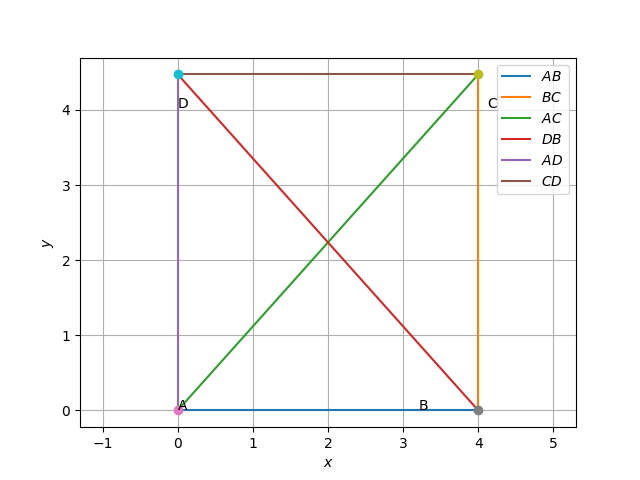
\includegraphics[scale=1]{fig.png} 
  
  Figure of construction
  	\end{center}
  	  
\bibliographystyle{ieeetr}
\end{document}